\documentclass[11pt,a4paper]{article}

\usepackage[utf8]{inputenc}
\usepackage[T1]{fontenc}
\usepackage{lmodern}
\usepackage{microtype}
\usepackage[a4paper, hmargin=0.73in, vmargin=0.63in]{geometry}
\usepackage{amsmath,amssymb}
\usepackage{booktabs}
\usepackage{tabularx}
\usepackage{graphicx}
\graphicspath{{../assets/}{./}}
\usepackage{xcolor}
\usepackage{hyperref}
\usepackage{float}
\usepackage{enumitem}
\usepackage{titlesec}
\usepackage{caption}

% Balanced, readable line and paragraph spacing
\linespread{1.12}
\setlength{\parskip}{5pt plus 1pt minus 1pt}
\setlength{\parindent}{0pt}

\titlespacing*{\section}{0pt}{10pt plus 2pt minus 2pt}{6pt plus 1pt minus 1pt}
\setlength{\intextsep}{10pt plus 2pt minus 2pt}
\setlength{\abovecaptionskip}{6pt}
\setlength{\belowcaptionskip}{4pt}

% Color definitions
\definecolor{primaryblue}{RGB}{20, 50, 110}
\definecolor{accentblue}{RGB}{41, 128, 185}

\hypersetup{
    colorlinks=true,
    linkcolor=primaryblue,
    citecolor=primaryblue,
    urlcolor=accentblue
}

% Clean plain page style (no top header, simple page number at bottom)
\pagestyle{plain}

\captionsetup{font=small, labelfont=bf}

\begin{document}

% =========================================================================
% PAGE 1: TITLE BLOCK & PART I
% =========================================================================

\begin{center}
    {\Large \textbf{\textcolor{primaryblue}{BO\u{G}AZ\.{I}\c{C}\.{I} UNIVERSITY}}}\\[0.25em]
    {\normalsize \textbf{Department of Computer Engineering}}\\[0.35em]
    {\large \textbf{CMPE 344: Computer Organization -- Prelab 3 Report}}\\[0.5em]
    \rule{\textwidth}{0.8pt}\\[0.45em]
    {\Large \textbf{Pipeline Waveform Analysis and Hazards on CORE-V Wally}}\\[0.4em]
    \rule{\textwidth}{0.8pt}\\[0.35em]
\end{center}

\begin{table}[H]
\centering
\renewcommand{\arraystretch}{1.2}
\begin{tabularx}{\textwidth}{@{}l X r@{}}
    \textbf{Group ID:} & \textbf{FF78\_G17} & \textbf{Date:} November 5, 2026 \\
    \textbf{Architecture:} & CORE-V Wally (\texttt{rv32i}, 5-Stage Pipeline) & \textbf{Tools:} Verilator \& GTKWave \\
\end{tabularx}
\end{table}

\section{Part I. Tracking the Instructions}

\begin{figure}[H]
    \centering
    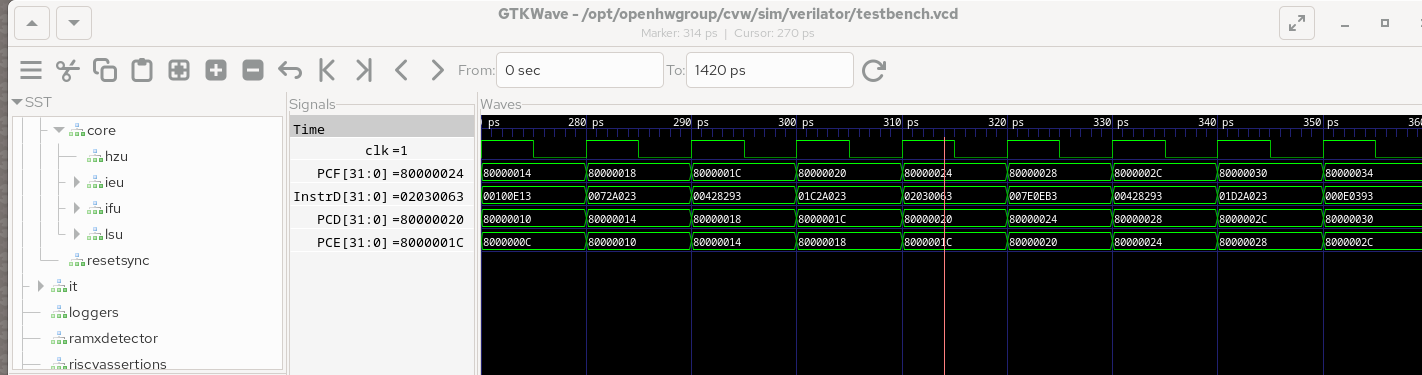
\includegraphics[width=\textwidth]{part1_wave.png}
    \caption{GTKWave waveform of the \texttt{fibonacci} simulation on CORE-V Wally (\texttt{rv32i}), showing \texttt{clk}, \texttt{PCF[31:0]}, \texttt{InstrD[31:0]}, \texttt{PCD[31:0]}, and \texttt{PCE[31:0]} with the marker placed in the clock cycle between $t = 310\text{ ps}$ and $t = 320\text{ ps}$ ($t = 314\text{ ps}$).}
    \label{fig:part1}
\end{figure}

Comparing the waveform during the selected clock cycle between $t = 310\text{ ps}$ and $t = 320\text{ ps}$ (Figure~\ref{fig:part1}) against the disassembled binary in \texttt{fibonacci.objdump} shows that the instruction currently being fetched at \texttt{PCF} and the instruction currently loaded in the Decode stage on \texttt{InstrD} are \textbf{not the same within the same clock cycle}; instead, they are separated by one clock cycle due to pipelining~\cite{harris2021}. Specifically, during the interval $t = 310\text{--}320\text{ ps}$, the Fetch stage Program Counter is \texttt{PCF = 0x80000024}, which in \texttt{fibonacci.objdump} corresponds to the arithmetic instruction \texttt{add t4, t3, t2} (encoded as machine code \texttt{0x007e0eb3}). During that same clock cycle ($t = 310\text{--}320\text{ ps}$), however, the instruction decoded on \texttt{InstrD} is \texttt{0x02030063}, which is the machine code for the conditional branch \texttt{beqz t1, 80000040 <DONE>} located at address \texttt{0x80000020}. Looking at the preceding clock cycle ($t = 300\text{--}310\text{ ps}$) on the waveform confirms that \texttt{PCF} was \texttt{0x80000020} one cycle earlier; on the rising clock edge at $t = 310\text{ ps}$, that address and its fetched instruction were latched into the Decode stage registers, producing \texttt{PCD = 0x80000020} and \texttt{InstrD = 0x02030063} during $t = 310\text{--}320\text{ ps}$ (while the earlier store instruction at \texttt{0x8000001c} moved into the Execute stage at \texttt{PCE = 0x8000001c}). Likewise, the instruction fetched from \texttt{PCF = 0x80000024} during $t = 310\text{--}320\text{ ps}$ is latched across the IF/ID pipeline register on the rising clock edge at $t = 320\text{ ps}$ and appears on \texttt{InstrD} as \texttt{0x007e0eb3} alongside \texttt{PCD = 0x80000024} during the next clock cycle ($t = 320\text{--}330\text{ ps}$), while \texttt{beqz t1, DONE} advances to the Execute stage (\texttt{PCE = 0x80000020}). Because inter-stage pipeline registers (\texttt{PCD} and \texttt{PCE}) pass instruction addresses and machine words forward by one stage on each rising clock edge, \texttt{PCF} always reflects the instruction being fetched from memory in the current cycle, whereas \texttt{InstrD} always holds the instruction at \texttt{PCD} that was fetched one cycle earlier.

% =========================================================================
% PART II
% =========================================================================

\section{Part II. Unexpected Instructions}

In \texttt{fibonacci.objdump}, the loop body ends at address \texttt{0x8000003c} with the unconditional jump instruction \texttt{j 80000020 <LOOP>} (machine code \texttt{0xfe5ff06f}), and the next sequential address in program memory is \texttt{0x80000040} under the label \texttt{DONE}, which holds the self-looping halt instruction \texttt{j 80000040 <DONE>} (machine code \texttt{0x0000006f}). In Wally's 5-stage pipeline, branch outcomes and jump target addresses are not determined until the instruction reaches the Execute (\texttt{E}) stage, two clock cycles after it is fetched~\cite{harris2021}. Because the Instruction Fetch Unit (\texttt{ifu}) must fetch an instruction on every clock cycle to keep all five pipeline stages utilized and sustain a throughput close to one instruction per cycle, it cannot stall and wait two cycles after every instruction just to check whether control flow will change. Instead, the \texttt{ifu} uses speculative sequential fetching: on each clock cycle, it assumes no branch or jump is taken (\textit{predict-not-taken}) and advances the Program Counter sequentially to \texttt{PCNextF = PCF + 4}~\cite{patterson2020}. Consequently, after \texttt{j LOOP} is fetched during $t = 370\text{--}380\text{ ps}$ (\texttt{PCF = 0x8000003c}) and latched into the Decode stage during $t = 380\text{--}390\text{ ps}$ (\texttt{PCD = 0x8000003c}, \texttt{InstrD = 0xfe5ff06f}), the Fetch stage automatically increments \texttt{PCF} to the next static memory address \texttt{0x80000040} and fetches \texttt{0x0000006f} (\texttt{DONE}). In the following cycle ($t = 390\text{--}400\text{ ps}$), as \texttt{j LOOP} enters the Execute stage (\texttt{PCE = 0x8000003c}), the sequentially fetched \texttt{0x0000006f} instruction enters the Decode stage (\texttt{PCD = 0x80000040}, \texttt{InstrD = 0x0000006f}) while \texttt{PCF} increments again to \texttt{0x80000044}. This speculative fetching mechanism is provided because the vast majority of executed instructions are sequential and conditional branches such as \texttt{beqz t1, DONE} (at \texttt{0x80000020}) are not taken during the first 10 iterations of the loop; fetching \texttt{PCF + 4} every cycle allows sequential code and untaken branches to execute without any stall penalty.

\begin{figure}[H]
    \centering
    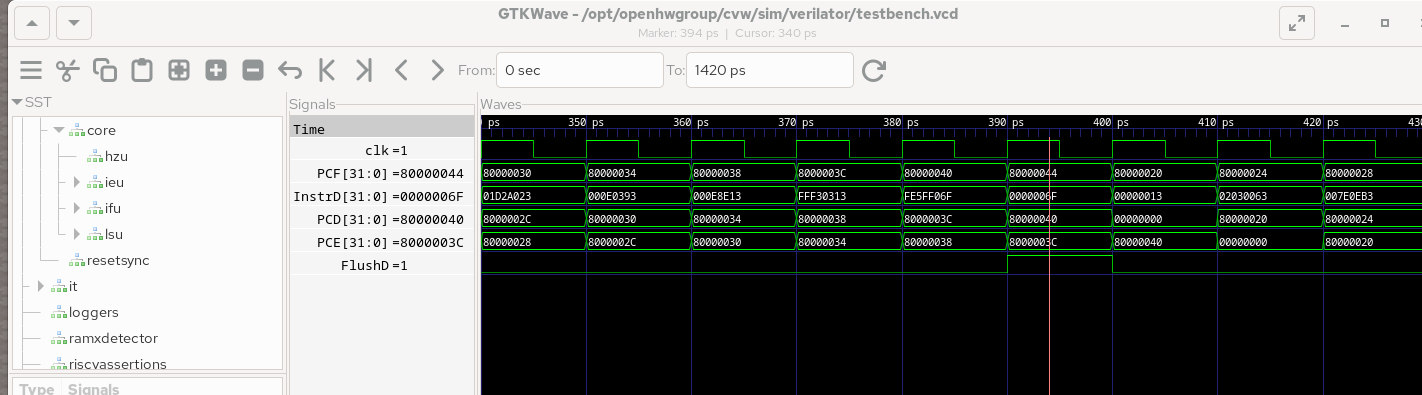
\includegraphics[width=\textwidth]{part2_wave.png}
    \caption{GTKWave waveform showing the wrong-path instruction \texttt{InstrD = 0000006F} (\texttt{DONE}) and \texttt{FlushD = 1} during $t = 390\text{--}400\text{ ps}$ ($t = 394\text{ ps}$ marker), followed by the pipeline flush and jump redirection in $t = 400\text{--}410\text{ ps}$.}
    \label{fig:part2}
\end{figure}

During the clock cycle $t = 390\text{--}400\text{ ps}$, the unconditional jump \texttt{j 80000020 <LOOP>} is in the Execute stage (\texttt{PCE = 0x8000003c}), where the processor resolves the jump condition and computes the target address \texttt{0x80000020}. Because the two instructions that were speculatively fetched after the jump (currently at \texttt{PCF = 0x80000044} in Fetch and \texttt{PCD = 0x80000040}, \texttt{InstrD = 0x0000006f} in Decode) lie on the wrong execution path and must not be allowed to alter architectural state, the Hazard Unit (\texttt{hzu}) asserts \texttt{FlushD = 1} (as well as \texttt{FlushE = 1}) throughout $t = 390\text{--}400\text{ ps}$~\cite{harris2021}. At the clock cycle right after \texttt{FlushD} is high ($t = 400\text{--}410\text{ ps}$, Figure~\ref{fig:part2}), three actions occur on the rising clock edge at $t = 400\text{ ps}$: first, the asserted \texttt{FlushD} signal synchronously clears the IF/ID pipeline registers, discarding the wrong-path instruction fetched from \texttt{0x80000044}, resetting \texttt{PCD} to \texttt{0x00000000}, and replacing \texttt{InstrD} with a \texttt{nop} bubble (\texttt{addi x0, x0, 0}, encoded as \texttt{0x00000013}); second, the wrong-path \texttt{0x0000006f} instruction advancing from Decode into Execute (\texttt{PCE = 0x80000040}) is simultaneously flushed into a \texttt{nop} (whose address becomes \texttt{0x00000000} in the next cycle) so that it performs no register writes or memory operations; and third, \texttt{PCF} is redirected to the jump target address \texttt{0x80000020} (\texttt{LOOP}) to fetch the loop header instruction \texttt{beqz t1, DONE} (\texttt{0x02030063}), while \texttt{FlushD} deasserts back to \texttt{0}. In the subsequent cycle ($t = 410\text{--}420\text{ ps}$), \texttt{0x02030063} is latched into \texttt{InstrD} with \texttt{PCD = 0x80000020}, resuming execution at the start of the second loop iteration.

% =========================================================================
% PART III
% =========================================================================

\section{Part III. Data Hazard}

In the Part~III template program, \texttt{lw x6, 0(x5)} at \texttt{0x80000014} loads the first array element (\texttt{arr[0] = 1111}) into register \texttt{x6} and is separated by a single \texttt{nop} (\texttt{0x80000018}) from the dependent instruction \texttt{add x8, x6, x6} at \texttt{0x8000001c}. This sequence creates a \textbf{Read-After-Write (RAW) data hazard} on \texttt{x6}. As shown in Figure~\ref{fig:part3}, during $t = 290\text{--}300\text{ ps}$, \texttt{lw x6, 0(x5)} is in Execute (\texttt{PCE = 0x80000014}, \texttt{Rs1E = 05}, \texttt{RdE = 06}) while \texttt{add x8, x6, x6} is fetched (\texttt{PCF = 0x8000001c}). During $t = 300\text{--}310\text{ ps}$, when \texttt{add x8, x6, x6} is in Decode (\texttt{PCD = 0x8000001c}) reading \texttt{x6} from the register file, \texttt{lw x6, 0(x5)} is still in the Memory stage (\texttt{RdM = 06}) reading data memory, so the register file still outputs the old value of \texttt{x6} (\texttt{0}). In the third clock cycle shown ($t = 310\text{--}320\text{ ps}$), \texttt{lw x6, 0(x5)} reaches Writeback (\texttt{RdW = 06}) at the exact same clock cycle that \texttt{add x8, x6, x6} enters Execute (\texttt{PCE = 0x8000001c}, \texttt{Rs1E = 06}, \texttt{Rs2E = 06}, \texttt{RdE = 08}).

\begin{figure}[H]
    \centering
    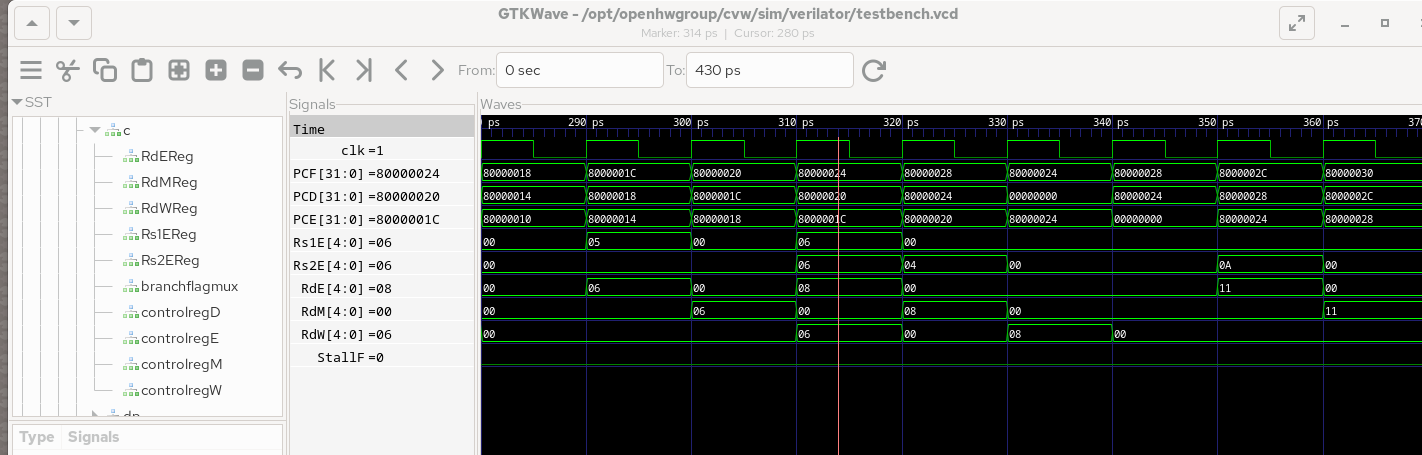
\includegraphics[width=\textwidth]{part3_wave.png}
    \caption{GTKWave waveform for Part~III at $t = 310\text{--}320\text{ ps}$ ($t = 314\text{ ps}$ marker), where \texttt{add x8, x6, x6} is in the Execute stage (\texttt{PCE = 8000001C}, \texttt{Rs1E = 06}, \texttt{Rs2E = 06}, \texttt{RdE = 08}) in the same cycle that \texttt{lw x6, 0(x5)} is in the Writeback stage (\texttt{RdW = 06}) with \texttt{StallF = 0}.}
    \label{fig:part3}
\end{figure}

The fundamental mechanism that allows an instruction in the Execute stage to use a register value in the same clock cycle that it is changing in the Writeback stage, without stalling the pipeline (\texttt{StallF = 0}), is \textbf{Data Forwarding (also called Bypassing)}~\cite{harris2021,patterson2020}. Without forwarding, the ALU in Execute would only receive operand values read from the register file during Decode, which are stale whenever an earlier instruction in Memory or Writeback has not yet written its result back to the register file. Data forwarding resolves this hazard in hardware by routing direct combinational bypass paths from the outputs of the Memory (\texttt{M}) and Writeback (\texttt{W}) stages back to 3-to-1 multiplexers placed at the ALU inputs in the Execute (\texttt{E}) stage~\cite{harris2021}. The Hazard Unit compares the Execute source registers (\texttt{Rs1E} and \texttt{Rs2E}) against the destination registers in Memory (\texttt{RdM}) and Writeback (\texttt{RdW}):
{\small
\begin{equation*}
\texttt{ForwardAE} = \begin{cases}
\texttt{10} & \text{if } (\texttt{Rs1E} == \texttt{RdM}) \land (\texttt{Rs1E} \neq 0) \land \texttt{RegWriteM} \;\; \text{(Forward ALU result from Memory stage)} \\
\texttt{01} & \text{else if } (\texttt{Rs1E} == \texttt{RdW}) \land (\texttt{Rs1E} \neq 0) \land \texttt{RegWriteW} \;\; \text{(Forward result from Writeback stage)} \\
\texttt{00} & \text{otherwise} \;\; \text{(Use register file value read in Decode stage)}
\end{cases}
\end{equation*}
}
(with identical logic generating \texttt{ForwardBE} for \texttt{Rs2E}). During $t = 310\text{--}320\text{ ps}$ in Figure~\ref{fig:part3}, the instruction in Memory is \texttt{nop} (\texttt{RdM = 00}), whereas the instruction in Writeback is \texttt{lw x6, 0(x5)} (\texttt{RdW = 06}, \texttt{RegWriteW = 1}). Because \texttt{Rs1E = 06 == RdW} and \texttt{Rs2E = 06 == RdW}, the Hazard Unit sets \texttt{ForwardAE = 01} and \texttt{ForwardBE = 01}. Both ALU input multiplexers bypass the old register file values from Decode and select the Writeback result bus (\texttt{ResultW = 1111}) directly, computing $1111 + 1111 = 2222$ during $t = 310\text{--}320\text{ ps}$ with no stall (\texttt{StallF = 0}). (When a consumer instruction is in \textit{Decode} while the producer is in \textit{Writeback}, a 5-stage pipeline also uses \textbf{split-phase register file access}, writing on the falling clock edge and reading combinationally in the second half of the cycle~\cite{harris2021,patterson2020}; when the consumer is in \textit{Execute} as in Figure~\ref{fig:part3}, \textbf{Writeback-to-Execute forwarding} supplies the operand directly to the ALU.)

% =========================================================================
% PART IV & REFERENCES
% =========================================================================

\section{Part IV. Load-Use Hazard}

\begin{figure}[H]
    \centering
    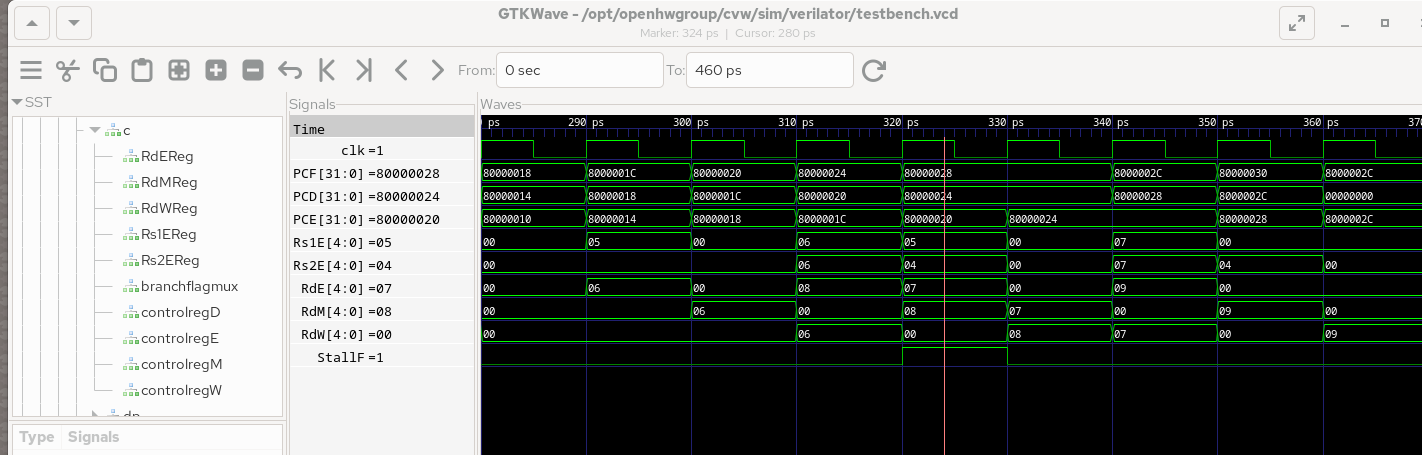
\includegraphics[width=\textwidth]{part4_wave.png}
    \caption{GTKWave waveform of \texttt{prelab3\_FF78\_G17.s} across $t = 320\text{--}350\text{ ps}$ ($t = 324\text{ ps}$ marker): \texttt{StallF = 1} is asserted during $t = 320\text{--}330\text{ ps}$ when \texttt{lw x7, 4(x5)} is in Execute (\texttt{PCE = 80000020}, \texttt{RdE = 07}) and \texttt{add x9, x7, x7} is in Decode (\texttt{PCD = 80000024}), stalling the pipeline during $t = 330\text{--}340\text{ ps}$.}
    \label{fig:part4}
\end{figure}

To implement the most simplistic load-use hazard inside the template block of \texttt{prelab3\_FF78\_G17.s}, we added \texttt{lw x7, 4(x5)} (at \texttt{0x80000020}, loading the second array element \texttt{arr[1] = 2222} into \texttt{x7}) immediately followed by \texttt{add x9, x7, x7} (at \texttt{0x80000024}, using \texttt{x7} as both \texttt{Rs1} and \texttt{Rs2}) with no \texttt{nop} between them. Unlike an arithmetic instruction whose result is ready at the end of the Execute (\texttt{E}) stage, a load instruction (\texttt{lw}) only computes the effective memory address (\texttt{x5 + 4}) in Execute and does not receive the loaded word from data memory until the end of the \textbf{Memory (\texttt{M})} stage~\cite{harris2021,patterson2020}. Because the loaded data is not yet available at the end of Execute, forwarding alone cannot supply \texttt{x7} to an instruction that enters Execute in the very next cycle, requiring a one-cycle stall. In Figure~\ref{fig:part4}, during $t = 320\text{--}330\text{ ps}$ ($t = 324\text{ ps}$ marker), \texttt{lw x7, 4(x5)} is in Execute (\texttt{PCE = 0x80000020}, \texttt{Rs1E = 05}, \texttt{RdE = 07}), the dependent \texttt{add x9, x7, x7} is in Decode (\texttt{PCD = 0x80000024}) requesting \texttt{x7}, and \texttt{j END} is in Fetch (\texttt{PCF = 0x80000028}). Detecting that the instruction in Execute is a load whose destination register (\texttt{RdE = 07}) matches the Decode source operands, the Hazard Unit asserts \texttt{StallF = 1} (along with \texttt{StallD = 1} and \texttt{FlushE = 1}) during $t = 320\text{--}330\text{ ps}$~\cite{harris2021}. Consequently, in the next clock cycle ($t = 330\text{--}340\text{ ps}$), \texttt{PCF} stays held at \texttt{0x80000028} (preventing a new instruction fetch) and \texttt{PCD} stays held at \texttt{0x80000024} (keeping \texttt{add x9, x7, x7} stalled in Decode for one cycle), while a \texttt{nop} bubble (\texttt{Rs1E = 00}, \texttt{Rs2E = 00}, \texttt{RdE = 00}) is inserted into Execute as \texttt{lw x7, 4(x5)} moves to the Memory stage (\texttt{RdM = 07}). At $t = 340\text{--}350\text{ ps}$, \texttt{lw x7, 4(x5)} enters Writeback (\texttt{RdW = 07}), \texttt{StallF} returns to \texttt{0}, and \texttt{add x9, x7, x7} enters Execute (\texttt{PCE = 0x80000024}, \texttt{Rs1E = 07}, \texttt{Rs2E = 07}, \texttt{RdE = 09}), receiving the loaded value of \texttt{x7} from Writeback via forwarding.

\vspace{0.1em}
\begin{thebibliography}{9}
\small
\setlength{\itemsep}{2pt}
\bibitem{harris2021}
S.~L. Harris and D.~Harris, \emph{Digital Design and Computer Architecture: RISC-V Edition}, Morgan Kaufmann / Elsevier, 2021, Section~7.5 (``Pipelined Processor'' and ``Hazards''), pp.~426--462.

\bibitem{patterson2020}
D.~A. Patterson and J.~L. Hennessy, \emph{Computer Organization and Design RISC-V Edition: The Hardware Software Interface}, 2nd~ed., Morgan Kaufmann, 2020, Sections~4.7--4.8 (``Data Hazards: Forwarding versus Stalling'' and ``Control Hazards''), pp.~303--325.
\end{thebibliography}

\end{document}
